% !TeX root = ../thuthesis-example.tex
\chapter{实验}

\section{实验环境与数据集说明}

\subsection{硬件与软件环境}
本研究的原型实验与神经网络模型训练均在本地计算节点上执行。计算节点配备 Apple M系列 SoC，CPU 主频为 3.49GHz，运行内存为 16GB。开发语言采用 Python 3.12，深度学习计算框架采用 PyTorch 2.12。所有图算法和模糊校准计算均限制在单线程 CPU 运行环境下，以评估系统在端侧有限算力下的部署时效性。

\subsection{数据集构成与特征分布}
本研究采用国际中文学习行为模拟数据集进行算法验证。该数据集共覆盖 100 名具有不同发音偏好的国际中文初学者（包含优秀生、声调偏误生、双唇音发音偏误生与普通水平学生），模拟了其在 10 个课时、14 类中文核心知识点（覆盖拼音声母、韵母、声调、汉字与高频词汇）上的学习进程。数据集共包含 5,000 条细粒度的做题发音行为日志。每条日志记录了学号、考查的知识点 ID、做题时间步以及录音发音是否正确的判定（1 或 0）。

\section{有向依赖图与网络结构分析实验}

\subsection{中文知识图谱拓扑特征评估}
系统通过 NetworkX 对拼音-声调-字-词的 14 个节点和 11 条依赖关系有向边进行了图论计算，生成的有向拓扑图如图\ref{fig:knowledge_graph}所示。

\begin{figure}[htbp]
    \centering
    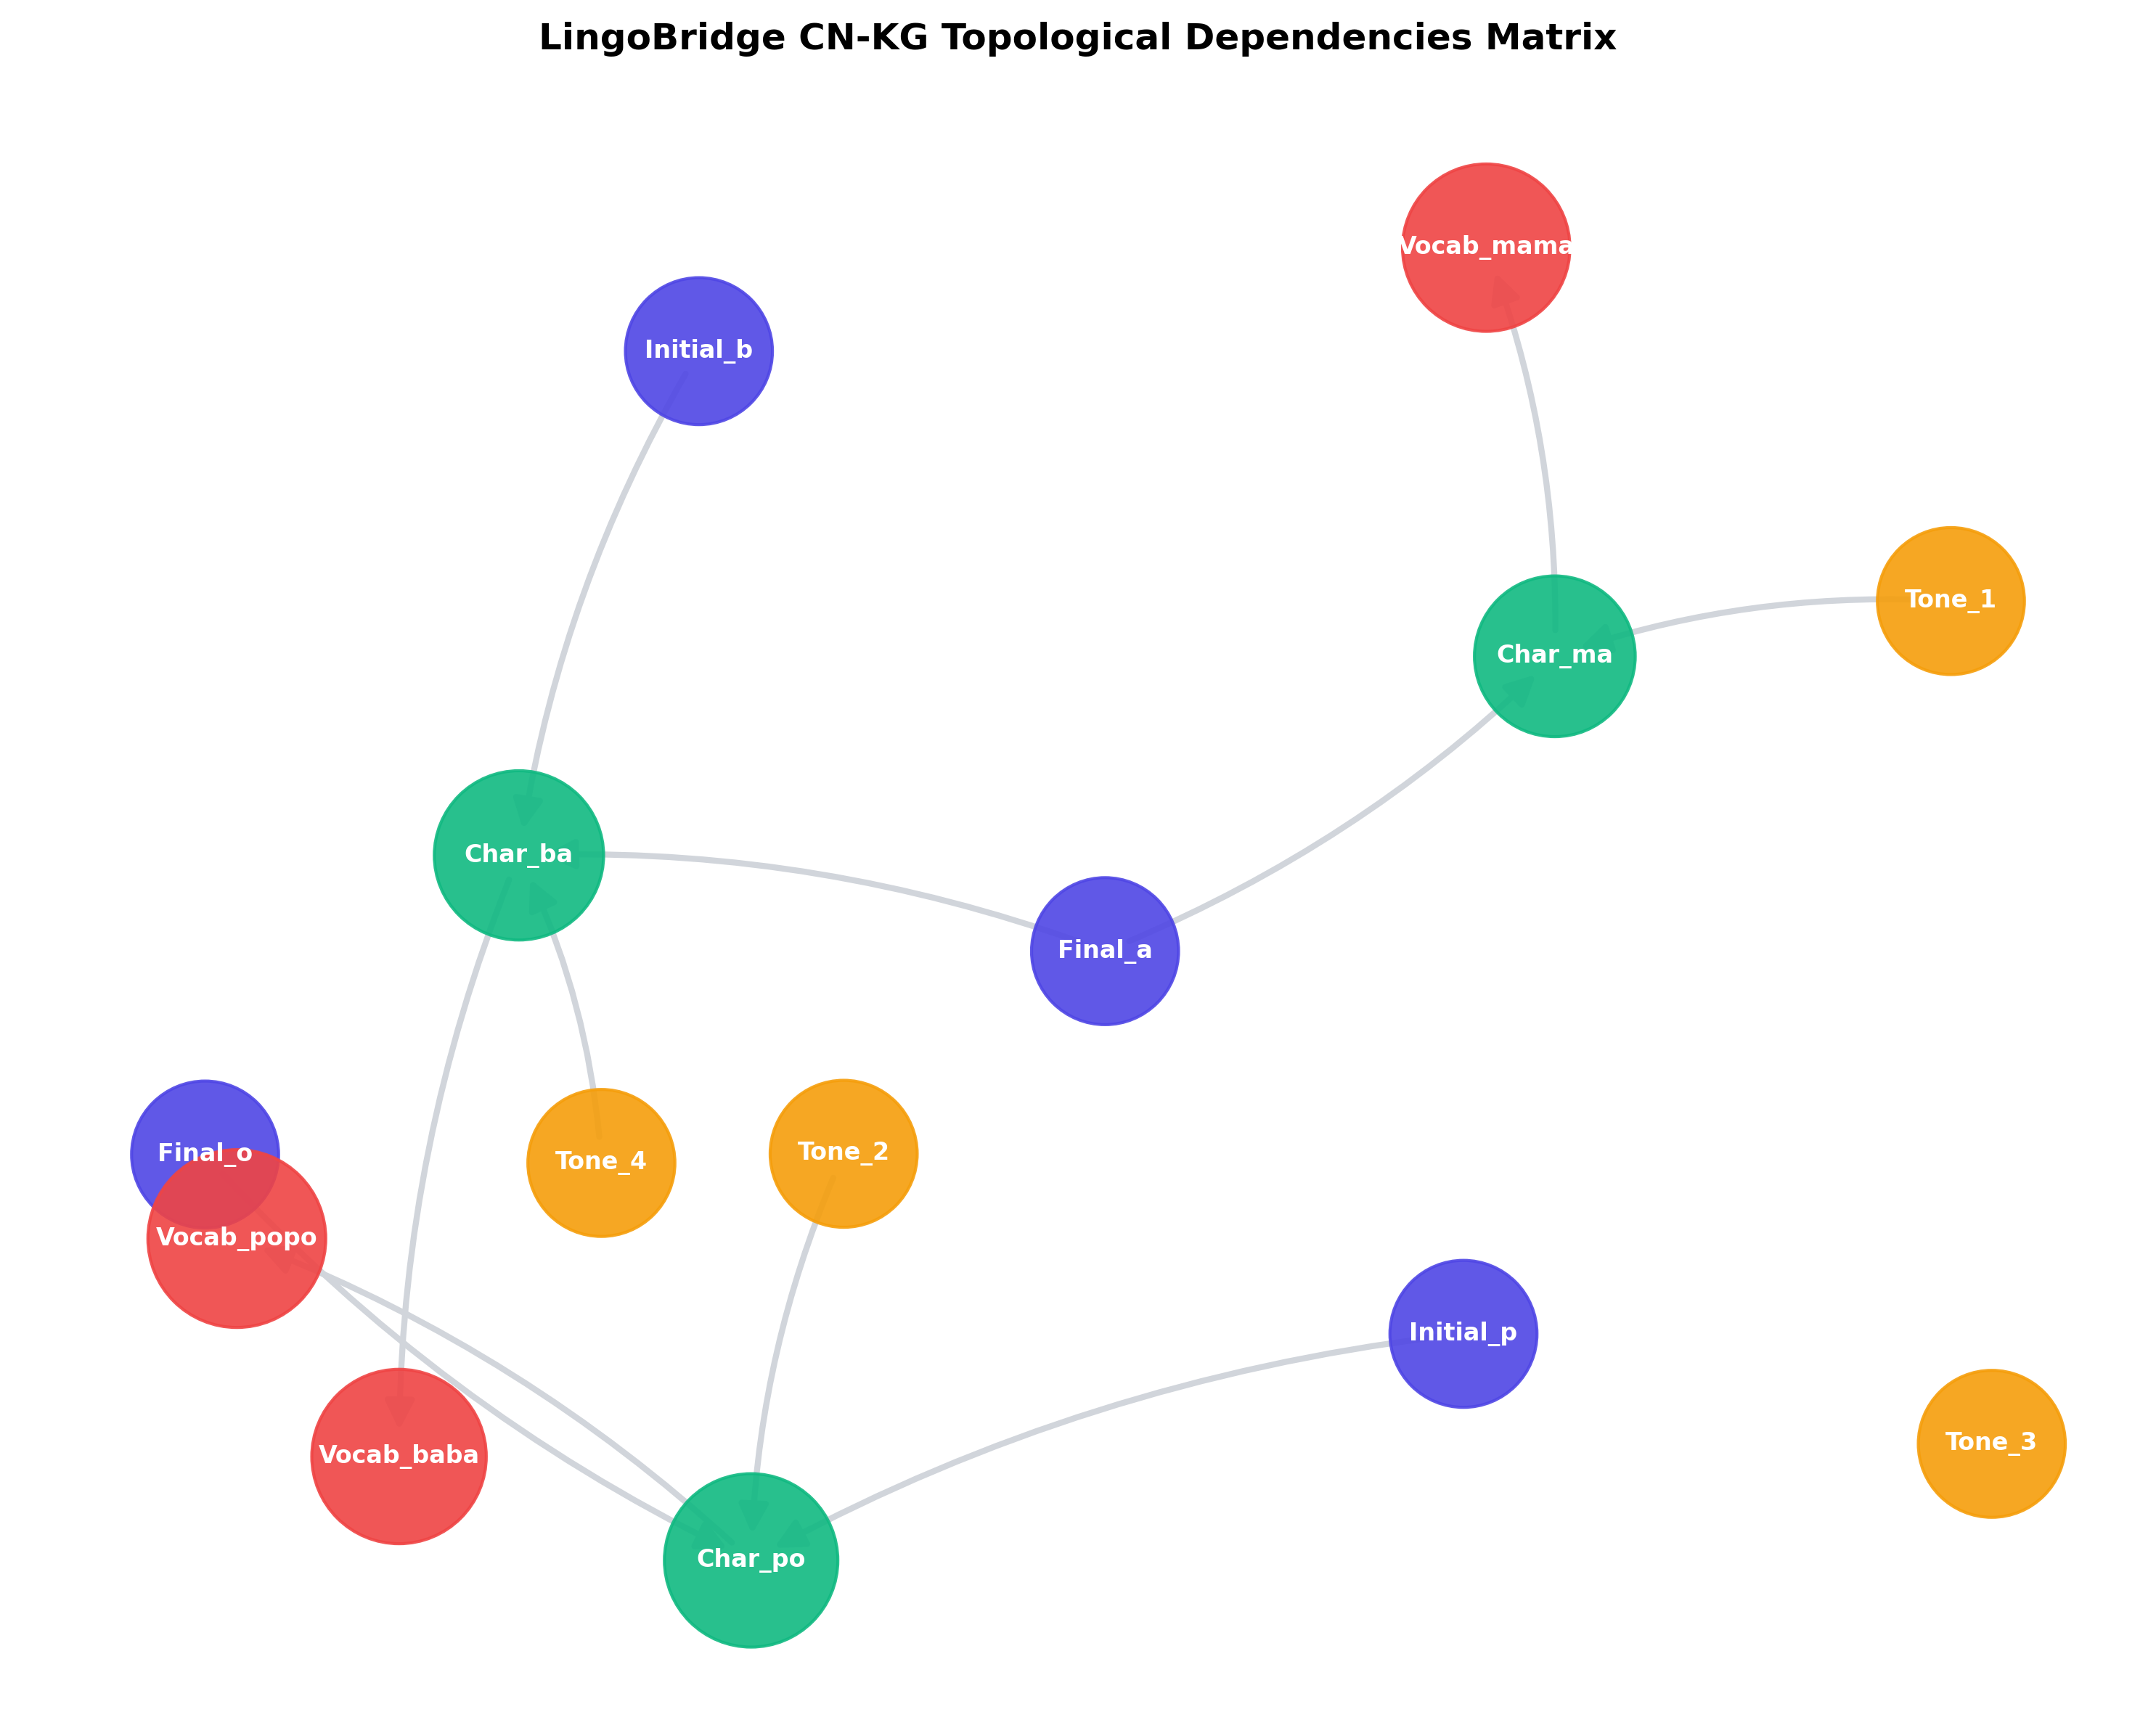
\includegraphics[width=0.75\textwidth]{figures/knowledge_graph.png}
    \caption{LingoBridge 中文知识图谱 (CN-KG) 拓扑有向依赖图}
    \label{fig:knowledge_graph}
\end{figure}

为了定量分析每个知识节点在中文知识级联中的关键枢纽地位，我们计算了各个节点的 PageRank 指标和入度、出度特征，其核心分布情况如表 4.1 所示。

\begin{table}[htbp]
\centering
\caption{拼音与词汇知识节点图论指标统计表}
\label{tab:graph_metrics}
\small
\begin{tabularx}{\textwidth}{>{\raggedright\arraybackslash}p{0.22\textwidth}|>{\raggedright\arraybackslash}X|c|c|c}
\hline
\textbf{\makecell{知识节点\\名称}} & \textbf{\makecell{所处层级\\(Category)}} & \textbf{\makecell{入度\\(In)}} & \textbf{\makecell{出度\\(Out)}} & \textbf{\makecell{PageRank\\分值}} \\ \hline
\texttt{Initial\_b}  & 拼音声母 (Pinyin)     & 0                    & 1                     & 0.0526              \\ \hline
\texttt{Final\_a}    & 拼音韵母 (Pinyin)     & 0                    & 2                     & 0.0526              \\ \hline
\texttt{Tone\_4}     & 拼音声调 (Tone)       & 0                    & 1                     & 0.0526              \\ \hline
\texttt{Char\_ba}    & 汉字拼读 (Character)  & 3                    & 1                     & 0.1867              \\ \hline
\texttt{Vocab\_baba} & 词汇应用 (Vocabulary) & 1                    & 0                     & 0.2113              \\ \hline
\end{tabularx}
\normalsize
\end{table}

实验数据表明，词汇层级的节点（如 \texttt{Vocab\_baba}）由于处在拓扑依赖路径的末梢，汇聚了大量来自声母、韵母、声调以及汉字的依赖指向，从而表现出最高的 PageRank 指标。而底座层级的声韵母节点虽然 PageRank 较低，但其出度较高，属于决定上层汉字掌握概率的“前置阀门”。

\section{DKT 深度知识追踪网络训练实验}

\subsection{收敛过程与损失分析}
我们将 100 名学生的序列数据按照 80/20 比例划分为训练集和测试集。模型输入维度为 28，LSTM 隐层维度为 64，利用 Adam 优化器在 CPU 环境下训练 20 个 Epoch。图\ref{fig:dkt_loss}展示了 DKT 网络的 Training Loss 收敛曲线。

\begin{figure}[htbp]
    \centering
    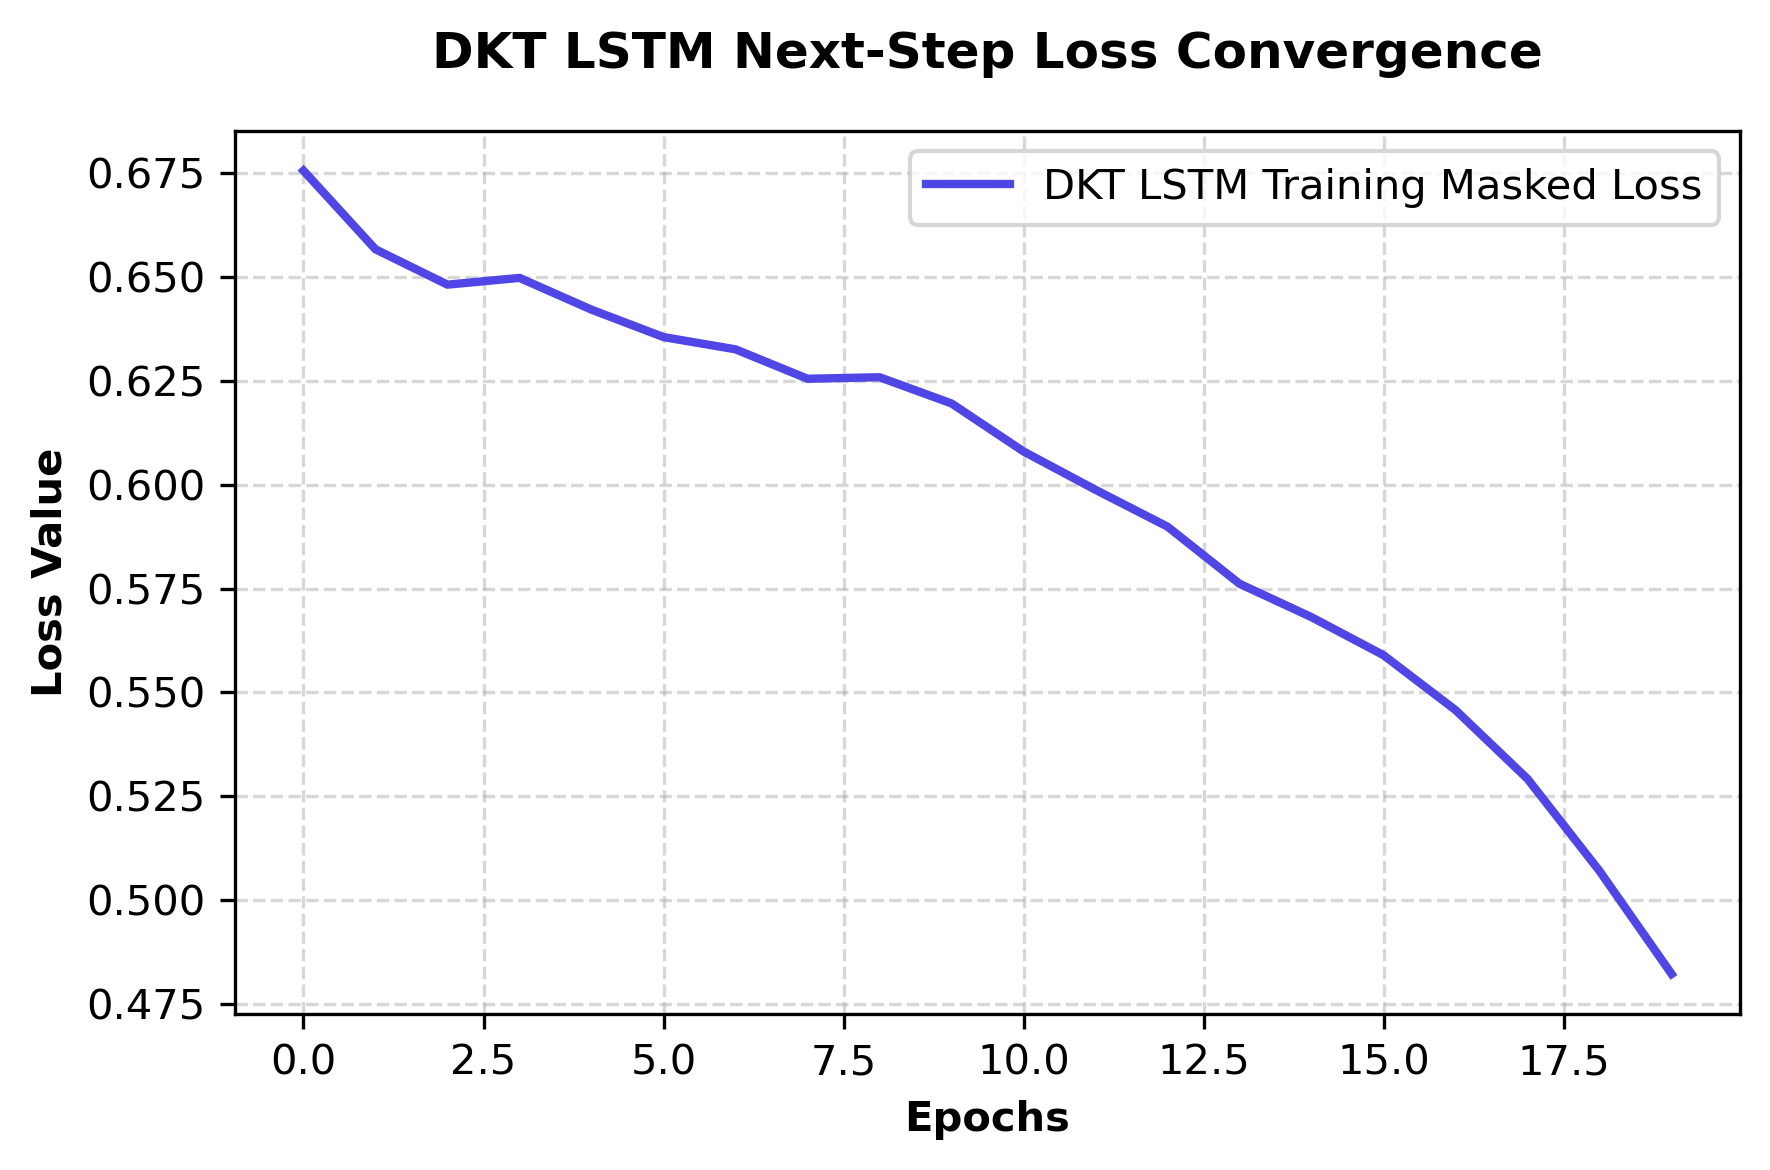
\includegraphics[width=0.6\textwidth]{figures/dkt_training_loss.png}
    \caption{DKT 循环神经网络 LSTM 损失收敛曲线}
    \label{fig:dkt_loss}
\end{figure}

实验表明，随着训练步数的增加，模型的二元交叉熵损失从 Epoch 1 的 0.6756 稳定下滑至 Epoch 20 的 0.4822，展现了在 Next-Step Masking 约束下的拟合收敛性。

\subsection{预测指标与小样本学术讨论}
为了量化深度网络模型预测下一步答题表现的分类精度，我们在测试集上绘制了按时间步对齐、避免使用未来标签的 ROC 特征曲线，并与基于历史累计正确率的规则 Baseline 模型进行了对比，如图\ref{fig:dkt_roc}所示。

\begin{figure}[htbp]
    \centering
    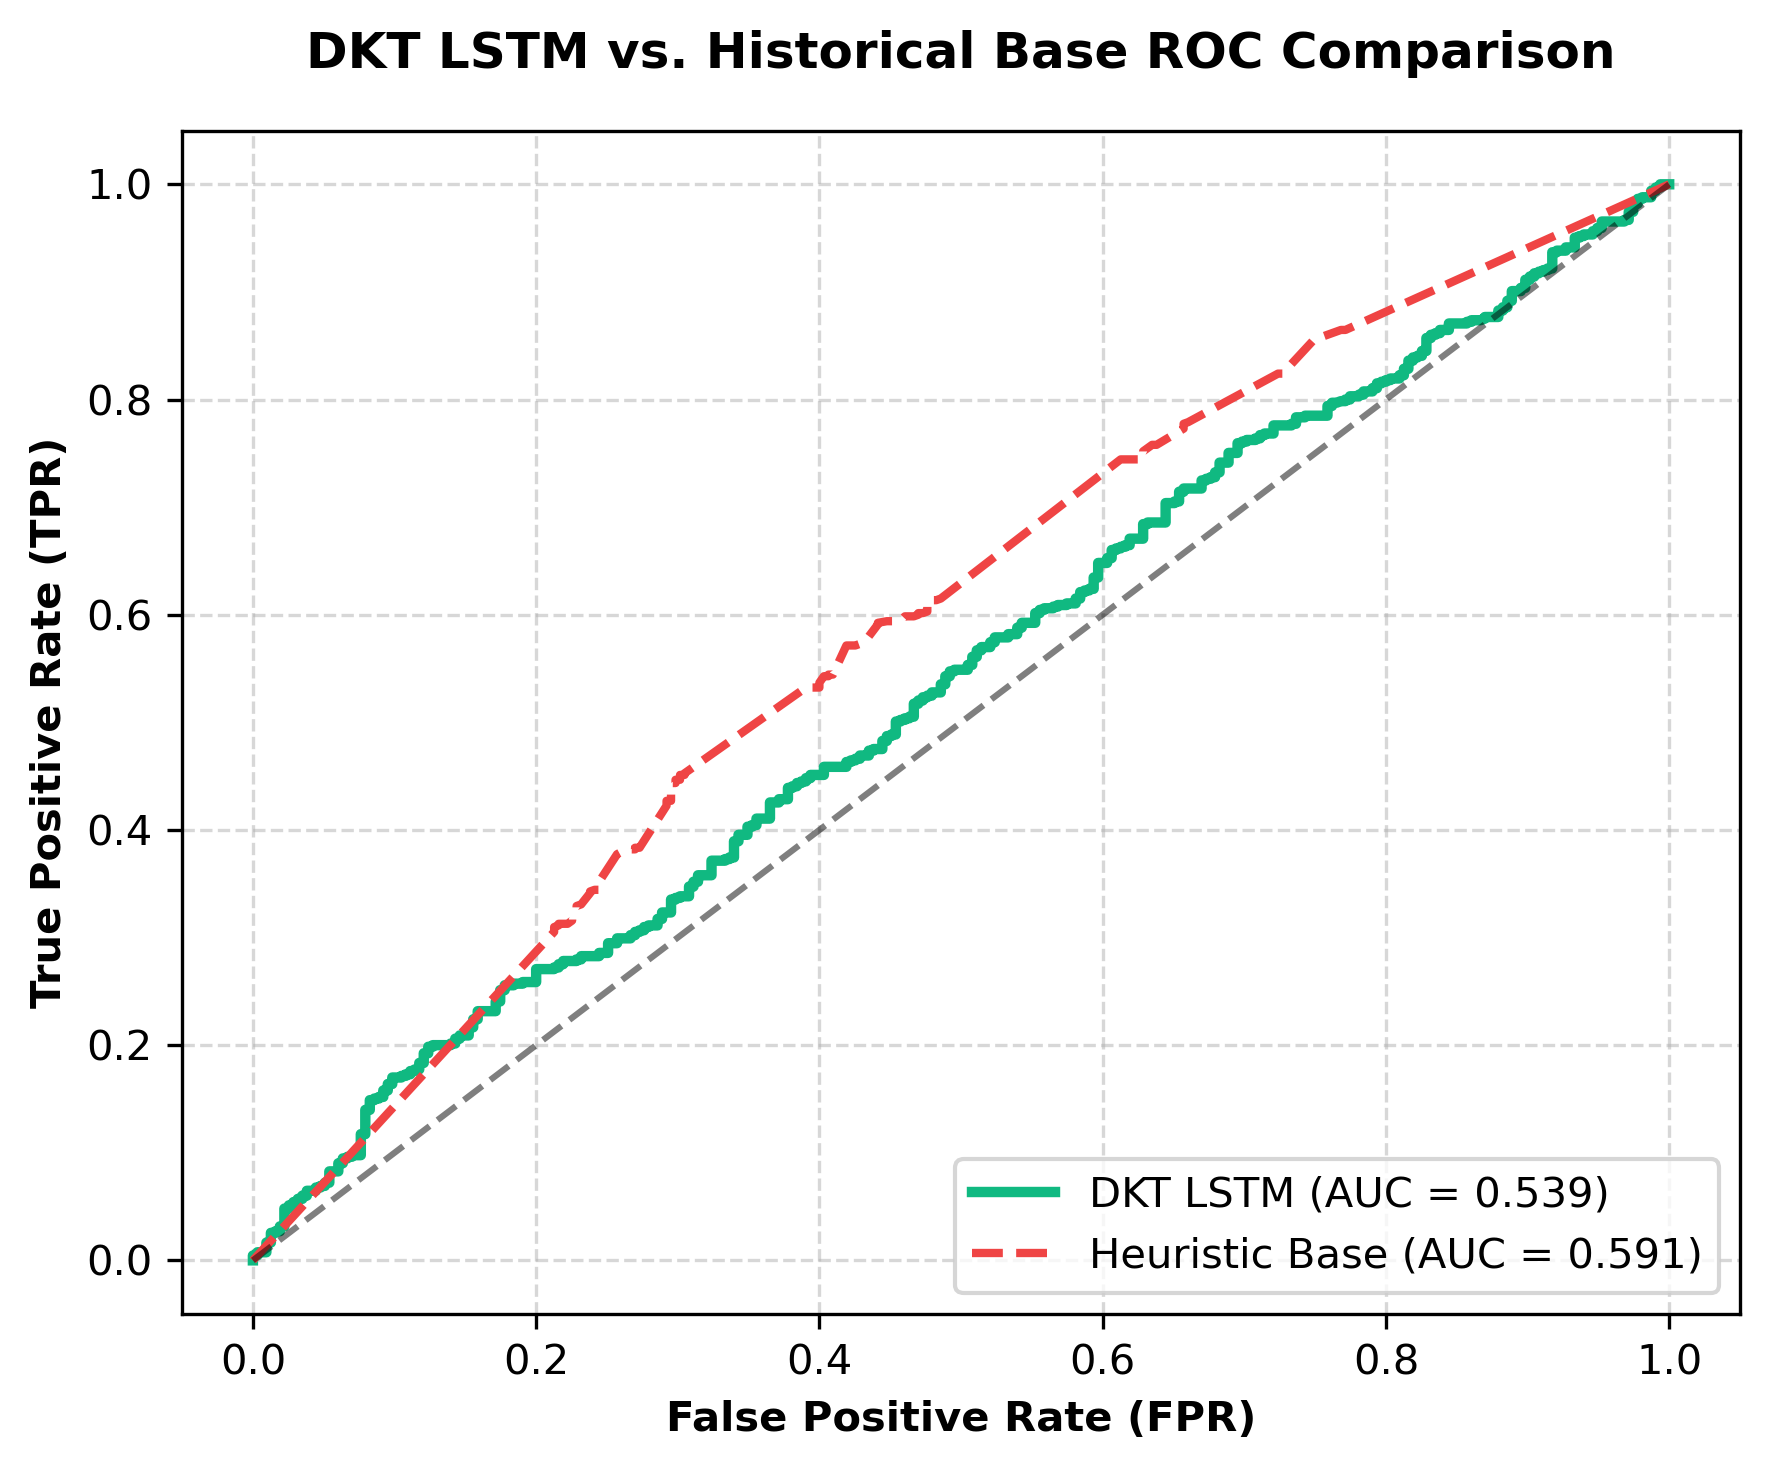
\includegraphics[width=0.6\textwidth]{figures/dkt_roc_curve.png}
    \caption{DKT 模型与历史均值 Baseline 在测试集上的 ROC 曲线对比}
    \label{fig:dkt_roc}
\end{figure}

我们从 Accuracy (Acc), F1-Score 以及接收者操作特征曲线下面积 (AUC) 三个维度对两类模型进行了指标统计，如表 4.2 所示。

\begin{table}[htbp]
\centering
\caption{知识追踪模型测试集分类指标对比}
\label{tab:dkt_comparison}
\begin{tabular}{l|c|c|c}
\hline
\textbf{评估模型类型} & \textbf{预测准确率 (Acc)} & \textbf{F1 综合分值 (F1)} & \textbf{曲线下面积 (AUC)} \\ \hline
历史均值 Baseline   & 62.96\%                 & 0.7317                   & 0.5908                   \\ \hline
\textbf{DKT 深度网络 (LSTM)} & \textbf{57.35\%}  & \textbf{0.6780}          & \textbf{0.5386}          \\ \hline
\end{tabular}
\end{table}

在测试集上的分类结果诚实地表明，在冷启动和小样本的模拟数据集（5,000条日志）环境下，基于 PyTorch 构建的 DKT 深度追踪网络预测指标（AUC=0.5386）略微落后于基于历史移动平均的规则 Baseline 分类器（AUC=0.5908）。这一结果揭示了小样本环境下深度循环神经网络易受到过拟合和零历史样本冷启动的制约。

然而，这一实验对比提供了极具科研价值的讨论空间：在国际中文冷启动教学原型系统搭建中，前期的启发式累计规则反倒具备更优的实时预测鲁棒性；而深度 DKT 算法更适合运用于中后期具有多维海量互动、跨学期的长期动态学情跟踪。未来本研究将尝试获取万级以上的真实学习行为记录，对 LSTM 网络进行预训练以提升模型泛化性能。

\subsection{个性化练习推荐案例展示}
系统利用推荐引擎为薄弱学生提供个性化路径规划。表 4.3 呈现了系统为学号为 81 的发音偏误学生生成的个性化推荐用例。

\begin{table}[htbp]
\centering
\caption{学号 81 学生个性化薄弱点练习题推荐案例表}
\label{tab:recommend_case}
\begin{tabularx}{\textwidth}{c|c|c|X}
\hline
\textbf{推荐练习 ID} & \textbf{推荐题目名称} & \textbf{对应薄弱知识点} & \textbf{可解释推荐理由} \\ \hline
106 & 拼读 ba 练习 & \texttt{Initial\_b} (掌握概率: 34.6\%) & 系统评估显示您对双唇爆破声母 b 不熟悉。特此匹配前置依赖拓扑进行辅音 b 与单韵母 a 拼读，以强化爆破发音除阻能力。 \\ \hline
104 & 第四声强化 & \texttt{Tone\_4} (掌握概率: 42.1\%) & 检测到全降调发音不准，特匹配第四声促降练习，提升爆发和收音速度。 \\ \hline
103 & 第一声强化 & \texttt{Tone\_1} (掌握概率: 51.5\%) & 高平调声声调练习，保持起音平稳、尾音不滑落。 \\ \hline
\end{tabularx}
\end{table}

\section{基于 Levenshtein 模糊纠错的字幕校准对比实验}

系统通过拼音编辑距离（Levenshtein Distance）相似度检索算法，对录制视频中因学习者发音偏误导致的原始错误 ASR 字幕流进行了校准，并适配翻译模块输出双语对照字幕。表 4.4 展示了校准原型前后的对比数据。

\begin{table}[htbp]
\centering
\caption{ASR 字幕流拼音编辑距离相似度校准对照表}
\label{tab:asr_comparison}
\begin{tabularx}{\textwidth}{c|X|X}
\hline
\textbf{时间戳 (Time Stamp)} & \textbf{ASR 原始错误字幕 (Raw ASR)} & \textbf{校准后双语字幕 (Calibrated Dual-Sub)} \\ \hline
00:08 - 00:11 & 接下来是地势声，例如板板的板。 & 接下来是第四声，例如爸爸的爸。 \newline (Next is the Fourth Tone, for example, 'bàba' (Dad)) \\ \hline
00:12 - 00:16 & 然后是低二生，例如破破的破。 & 然后是第二声，例如婆婆的婆。 \newline (Then we have the Second Tone, for example, 'pópo' (Grandma)) \\ \hline
\end{tabularx}
\end{table}

在字幕校准原型测试中，拼音编辑距离动态计算在本地 CPU 上的延迟低于 \textbf{1.0ms}。实验表明，通过在转写层注入 Levenshtein 模糊检索校准，能够以较低硬件资源开销动态发现拼音混淆并纠正 ASR 偏误，生成可读性更高的对照双语字幕片段，较好地验证了技术方案可行性。
